\documentclass[]{article}

% Imported Packages
%------------------------------------------------------------------------------
\usepackage{amssymb}
\usepackage{amstext}
\usepackage{amsthm}
\usepackage{amsmath}
\usepackage{enumerate}
\usepackage{fancyhdr}
\usepackage[margin=1in]{geometry}
\usepackage{graphicx}
\usepackage{extarrows}
\usepackage{setspace}
\usepackage{float}
%------------------------------------------------------------------------------

% Header and Footer
%------------------------------------------------------------------------------
\pagestyle{plain}
\renewcommand\headrulewidth{0.4pt}
\renewcommand\footrulewidth{0.4pt}
%------------------------------------------------------------------------------

% Title Details
%------------------------------------------------------------------------------
\title{
  Erudite\\
  \large \emph{An educational content management system}\\
  \vspace{1em}
  High-Level Architectural Design
}
\author{
  SE 3A04: Software Design II -- Large System Design
  \\
  \begin{tabular}{ l l }
    Kelvin Lin*   & STUDENT-NUM \\
    Danish Khan   & STUDENT-NUM \\
    Puru Jetly    & STUDENT-NUM \\
    Terrance Yip  & STUDENT-NUM \\
    Varun Hooda   & STUDENT-NUM \\
  \end{tabular}
}
\date{}
%------------------------------------------------------------------------------

% Document
%------------------------------------------------------------------------------
\begin{document}

\maketitle
\newpage

\tableofcontents
\newpage

\section{Introduction}
\label{sec:introduction}
This section outlines the purpose and provides a system description of the
Erudite project; along with an overview of the contents and organization of
this high-level architectural design document.


\subsection{Purpose}
\label{sub:purpose}
The purpose of this document to define the use cases, layout the Analysis Class
Diagram, describe the Architectural Design, and finally document the class
responsibilities through collaboration cards. This document builds on top of
and extends the Software Requirements Specification document in that this
document describes the way in which the system will interact with the outside
world and how the subsystems will be architecturally and logically arranged.

The target audience for this document are the stakeholders (Dr. Ridha Khedri,
Andrew Le Clair and Michael Liut), and any current or future architects,
designers and developers of this project.


\subsection{System Description}
\label{sub:system_description}
The Erudite application is intended to be an educational content management
system for use in elementary school classrooms. The primary interface between
the user and the software system is through a device running the Android
operating system. This document defines the way in which the users will be
expected to interact with the system and how the application will be decomposed
into smaller subsystems to reduce the complexity and improve the
maintainability, flexibility of this system.

Specifically, the users of this system (application) are expected to perform a
set of events that will prompt the system to react. The decomposition will then
show how the subsystems will communicate among one another in order to
efficiently distribute the work and perform the required actions in response to
the user's actions.


\subsection{Overview}
\label{sub:overview}
The remainder of the document is organized into 4 sections: Use Case Diagram --
how the users and system will interact, Analysis Class Diagram -- the
subsystems that compose this entire application, Architectural Design -- the
layout of the subsystems into a well-understood software architecture, and
Class responsibility collaboration Cards -- description of the interactions
between the subsystems. Each section uses an appropriate notation and diagrams
to document the design decision and describe the details of the high-level
design of this system.


% End Section


\newpage

\section{Use Case Diagram}
\label{sec:use_case_diagram}
% Begin Section
The following diagram is an use case diagram for Erudite.\\

{
  \centering
  \includegraphics[scale=0.40]{"A2_Assets/Use Case Diagram"}
}

\newpage

\section{Analysis Class Diagram}
\label{sec:analysis_class_diagram}
% Begin Section
The following diagram is an analysis class diagram for Erudite.\\

{
  \centering
  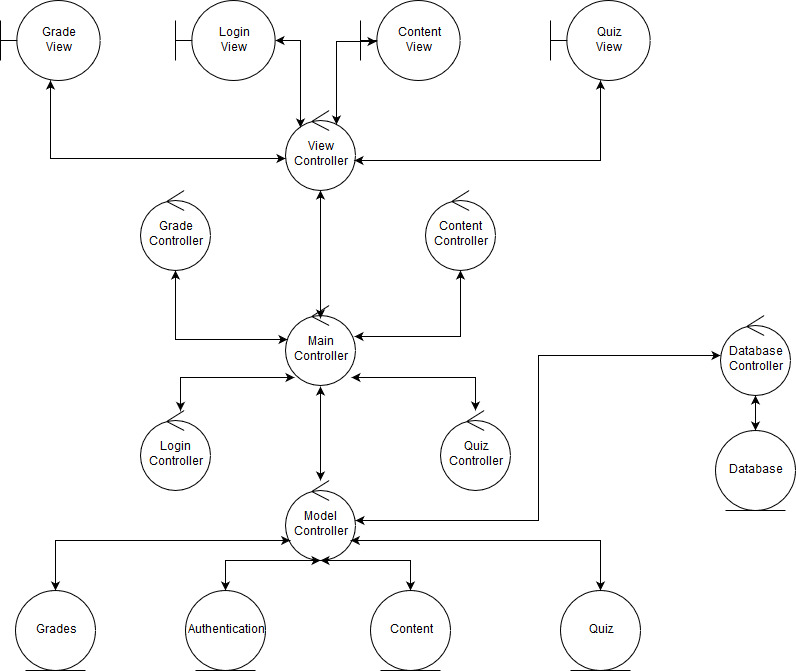
\includegraphics[scale=0.5]{A2_Assets/Analysis_Class_Diagrm_v2.jpg}
}


\section{Architectural Design}
\label{sec:architectural_design}
% Begin Section

{
  \centering
    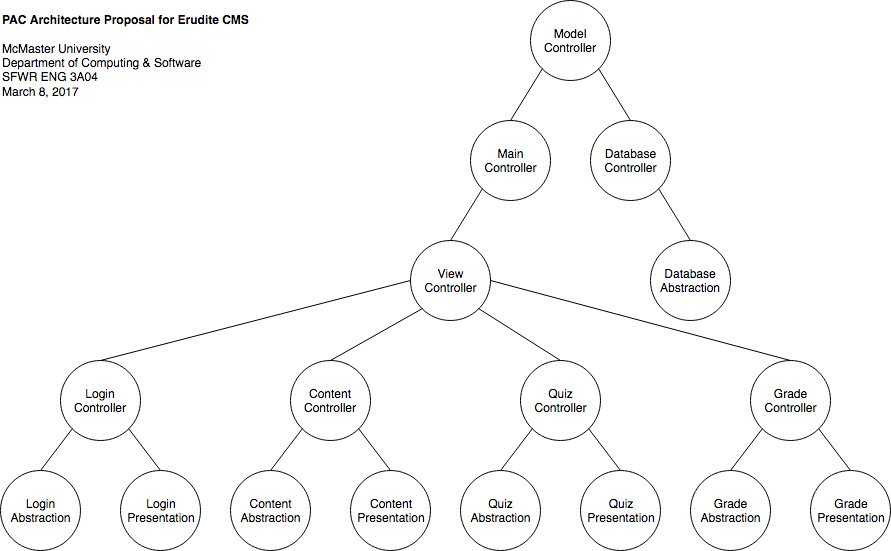
\includegraphics[scale=0.5]{A2_Assets/Structural_Class_Diagram_v2.jpg}
  \centerline{Structural Class Diagram}
}
System description.

\subsection{System Architecture}
\label{sub:system_architecture}
% Begin SubSection
Erudite will be built using the MVC-II architecture, where the system will be decomposed into views, controllers, models, and a database.

The MVC-II architecture was chosen because Erudite contains 3 main components: views, controllers (i.e. business logic), and data models. The MVC-II architecture allows for the separation of the 3 aforementioned components. This separation of concerns will allow for a seamless implementation of the application at the development phase, as different team members can be assigned to create different components of the overall system.

Furthermore, Erudite is used by 2 classes of users: teachers and students. Both classes of users use the same data; however, the way each class sees the data is different. For instance, students should only see their own grades, whereas teachers should see all of their students' grades. The MVC-II architecture allows for the different views to be implemented with the same set of data: the representation of the data does not need to change.  Moreover, additional views can be added without changing the rest of the system. Accordingly, the MVC-II architecture will be used.

%Add a structural architecture diagram here
% End SubSection

\subsection{Subsystems}
\label{sub:subsystems}
% Begin SubSection
\begin{enumerate}[a)]
	\item Provide a brief description of each subsystem. Be sure to document its
purpose and relationship to other subsystems.
\end{enumerate}
% End SubSection

% End Section

\section{Class Responsibility Collaboration (CRC) Cards}
\label{sec:class_responsibility_collaboration_crc_cards}
% Begin Section
This section should contain all of your CRC cards.

\begin{enumerate}[a)]
	\item Provide a CRC Card for each identified class
	\item Please use the format outlined in tutorial, i.e.,

  \begin{table}[H]
		\centering
		\begin{tabular}{|p{9cm}|p{3cm}|}
		\hline
		 \multicolumn{2}{|l|}{\textbf{Class Name:} LoginView} \\
		\hline
		\textbf{Responsibility:} & \textbf{Collaborators:} \\
		\hline
    Handles self-render request & ViewController \\
    \hline
    Requests to render ContentView & ViewController \\
    \hline
    Requests to render GradeView & ViewController \\
    \hline
    Requests to render QuizView & ViewController \\
    \hline
    Handles keyboard input & \\
    \hline
    Send login request to ViewController & ViewController \\
    \hline
    Send username and password pair to ViewController & ViewController \\
    \hline
    Prompt user if login request fails & ViewController \\
    \hline
    Request view change & ViewController \\
    \hline
		\end{tabular}
	\end{table}

  \begin{table}[H]
		\centering
		\begin{tabular}{|p{9cm}|p{3cm}|}
		\hline
		 \multicolumn{2}{|l|}{\textbf{Class Name:} ContentView} \\
		\hline
		\textbf{Responsibility:} & \textbf{Collaborators:} \\
		\hline
    Handles self-render request & ViewController \\
    \hline
    Requests to render LoginView & ViewController \\
    \hline
    Requests to render GradeView & ViewController \\
    \hline
    Requests to render QuizView & ViewController \\
    \hline
    Handles keyboard input & \\
    \hline
    Send course-content request to ViewController & ViewController \\
    \hline
    Send specific-file request to ViewController & ViewController \\
    \hline
    Display course content list & \\
    \hline
    Display specific file content list & \\
    \hline
    Request view change & ViewController \\
    \hline
		\end{tabular}
	\end{table}

  \begin{table}[H]
    \centering
    \begin{tabular}{|p{9cm}|p{3cm}|}
    \hline
     \multicolumn{2}{|l|}{\textbf{Class Name:} GradeView} \\
    \hline
    \textbf{Responsibility:} & \textbf{Collaborators:} \\
    \hline
    Handles self-render request & ViewController \\
    \hline
    Requests to render LoginView & ViewController \\
    \hline
    Requests to render ContentView & ViewController \\
    \hline
    Requests to render QuizView & ViewController \\
    \hline
    Handles keyboard input & \\
    \hline
    Display current course grades list & \\
    \hline
    Display current cumulative grade point average list & \\
    \hline
    Request view change & ViewController \\
    \hline
    \end{tabular}
  \end{table}

  \begin{table}[H]
    \centering
    \begin{tabular}{|p{9cm}|p{3cm}|}
    \hline
     \multicolumn{2}{|l|}{\textbf{Class Name:} QuizView} \\
    \hline
    \textbf{Responsibility:} & \textbf{Collaborators:} \\
    \hline
    Handles self-render request & ViewController \\
    \hline
    Requests to render LoginView & ViewController \\
    \hline
    Requests to render ContentView & ViewController \\
    \hline
    Requests to render GradeView & ViewController \\
    \hline
    Handles keyboard input & \\
    \hline
    Request course quiz list & ViewController \\
    \hline
    Request specific quiz & ViewController \\
    \hline
    Display course quiz list & \\
    \hline
    Display selected quiz & \\
    \hline
    Handles user answer selection & \\
    \hline
    Send quiz answers & ViewController \\
    \hline
    Request view change & ViewController \\
    \hline
    \end{tabular}
  \end{table}

	%quiz controller
	\begin{table}[H]
	\centering
		\begin{tabular}{|p{5cm}|p{5cm}|}
		\hline
		 \multicolumn{2}{|l|}{\textbf{Class Name: Quiz Controller}} \\
		\hline
		\textbf{Responsibility:} & \textbf{Collaborators:} \\
		\hline
		Knows Main Controller & \\
		\hline
		Receive quiz request from Main Controller & Main Controller \\
		\hline
		Send quiz request to Main Controller & Main Controller \\
		\hline
		Receive quiz result from Main Controller & Main Controller \\
		\hline
		Process quiz result from Main Controller & Main Controller \\
		\hline
		Receive student answer from Main Controller & Main Controller \\
		\hline
		Send request for solutions to Main Controller & Main Controller \\
		\hline
		Receive solutions from Main Controller & Main Controller \\
		\hline
		Mark quiz according to solution & \\
		\hline
		Send grade of quiz to Main Controller & Main Controller \\
		\hline

		\end{tabular}
	\end{table}

	%Grade Controller

	\begin{table}[H]
	\centering
		\begin{tabular}{|p{5cm}|p{5cm}|}
		\hline
		 \multicolumn{2}{|l|}{\textbf{Class Name: Grade Controller}} \\
		\hline
		\textbf{Responsibility:} & \textbf{Collaborators:} \\
		\hline
		Know Main Controller \\
		\hline
		Receive grade request from Main Controller & Main Controller \\
		\hline
		Send grade response to Main Controller & Main Controller \\
		\hline
		Receive grades from Main Controller & Main Controller \\
		\hline
		Process grades & \\
		\hline
		Send grades to Main Controller & Main Controller \\
		\hline
		\end{tabular}
	\end{table}

		%Model Controller

	\begin{table}[H]
	\centering
		\begin{tabular}{|p{5cm}|p{5cm}|}
		\hline
		 \multicolumn{2}{|l|}{\textbf{Class Name: Model Controller}} \\
		\hline
		\textbf{Responsibility:} & \textbf{Collaborators:} \\
		\hline
		Knows Main Controller & \\
		\hline
		Knows Database Controller & \\
		\hline
		Knows Grades Entity & \\
		\hline
		Know Authentication Token Entity & \\
		\hline
		Knows Content Entity & \\
		\hline
		Knows Quiz Entity & \\
		\hline
		Receive encrypted username and password & Main Controller \\
		\hline
		Send to Database Handler & Database Controller \\
		\hline
		Receive response object from Database Handler & Database Controller \\
		\hline
		Send response object from Database and return to Main Controller & Main \\
		\hline
		Receive authentication token storage request & Main Controller \\
		\hline
		Store authentication token & Authentication Token Entity \\
		\hline
		Receive content request & Main \\
		\hline
		Get authentication token & Authentication Token Entity \\
		\hline
		Send content request and authentication token & Database Controller \\
		\hline
		Receive content response & Database Controller \\
		\hline
		Send content response & Main Controller \\
		\hline
		Receive quiz request & Main Controller \\
		\hline
		Get authentication token & Authentication Token Entity \\
		\hline
		Send quiz request and authentication token & Database Controller\\
		\hline
		Receive quiz response & Database Controller \\
		\hline
		Send quiz response & Main Controller \\
		\hline
		Receive quiz solution request & Main Controller \\
		\hline
		Get authentication token & Authentication Token Entity \\
		\hline
		Send quiz solution request and authentication token & Database Controller \\
		\hline
		Receive quiz grade response & Database Controller \\
		\hline
		Send quiz grade response & Main \\
		\hline
		Receive grades request & Main \\
		\hline
		Get authentication token & Authentication Model \\
		\hline
		Send grades request and authentication token & Database Controller \\
		\hline
		Receive grades response & Database Controller \\
		\hline
		Send grades response & Main \\
		\hline
		\end{tabular}
	\end{table}

		%Database Controller

	\begin{table}[H]
	\centering
		\begin{tabular}{|p{5cm}|p{5cm}|}
		\hline
		 \multicolumn{2}{|l|}{\textbf{Class Name: Database Controller}} \\
		\hline
		\textbf{Responsibility:} & \textbf{Collaborators:} \\
		\hline
		Knows Model Controller & \\
		\hline
		Knows Database Entity & \\
		\hline
		Receive encrypted username and password from model handler & Model Handler \\
		\hline
		Verify username and password with the database & Database \\
		\hline
		Send response object to the model handler & Model Controller \\
		\hline
		Receive content request and authentication token & Model Controller \\
		\hline
		Grab content from database & Database \\
		\hline
		Send content response & Model Controller \\
		\hline
		Receive quiz request and authentication token & Model Controller \\
		\hline
		Grab quiz from database & Database \\
		\hline
		Send quiz response & Model Controller \\
		\hline
		Receive quiz solution request and authentication token & Model 		Controller \\
		\hline
		Grab quiz solution from database & Database \\
		\hline
		Send quiz solution response & Model Controller \\
		\hline
		Receive grade update request and authentication token & Model Controller \\
		\hline
		Update grades from database & Database \\
		\hline
		Receive grade request and authentication token & Model 	Controller \\
		\hline
		Grab grades from database & Database \\
		\hline
		Send grades response & Model Controller \\
		\hline
		\end{tabular}
	\end{table}

\end{enumerate}
% End Section


\newpage
\appendix
\section{Division of Labour}
\label{sec:division_of_labour}
\begin{description}
  \item [Kelvin Lin ]
  \item{Foo}
  \hfill \rule{2in}{0.1pt}
  \\\\

  \item [Danish Khan]
  \item{CRC Cards}
  \item{Structural Class Diagram}
  \hfill \rule{2in}{0.1pt}
  \\\\

  \item [Puru Jetly]
  \item{Baz}
  \hfill \rule{2in}{0.1pt}
  \\\\

  \item [Terrance Yip]
  \item{Qux}
  \hfill \rule{2in}{0.1pt}
  \\\\

  \item [Varun Hooda]
  \item{Section 1 Introduction}
  \item{Revision to use case diagram}
  \hfill \rule{2in}{0.1pt}
  \\\\
\end{description}


% \newpage
% \section*{IMPORTANT NOTES}
% \begin{itemize}
%   \item You do \underline{NOT} need to provide a text explanation of each
%   diagram; the diagram should speak for itself
%   \item Please document any non-standard notations that you may have used
%   \begin{itemize}
%     \item \emph{Rule of Thumb}: if you feel there is any doubt surrounding
%     the meaning of your notations, document them
%   \end{itemize}
%   \item Some diagrams may be difficult to fit into one page
%   \begin{itemize}
%     \item It is OK if the text is small but please ensure that it is readable
%     when printed
%     \item If you need to break a diagram onto multiple pages, please adopt a
%     system of doing so and thoroughly explain how it can be reconnected from
%     one page to the next; if you are unsure about this, please ask about it
%   \end{itemize}
%   \item Please submit the latest version of Deliverable 1 with Deliverable 2
%   \begin{itemize}
%     \item It does not have to be a freshly printed version; the latest marked
%     version is OK
%   \end{itemize}
%   \item If you do \underline{NOT} have a Division of Labour sheet, your
%   deliverable will \underline{NOT} be marked
% \end{itemize}


\end{document}
%------------------------------------------------------------------------------
